\documentclass[pdftex,11pt]{article}
\usepackage[pdftex]{graphicx}
\usepackage{enumerate}
\usepackage{amsmath}
\usepackage{amssymb}
\usepackage{multicol}
\usepackage{algpseudocode}
\usepackage{algorithm}
\usepackage{hyperref}
\usepackage{ listings}
\title{COMP 540 - Homework 3}
\author{Guangyuan Yu (gy12) right now I don't have a teammates}
\date{19/2/2017}
\DeclareMathOperator*{\argmax}{argmax}
\DeclareMathOperator*{\MAP}{MAP}
\begin{document}
\maketitle

\section{MAP and MLE Parameter Estimation}
\subsection{Deriving a $\theta^{*}$ Estimate}

\begin{align*}
\theta^{*} &= \argmax_\theta P(D|\theta) = \prod_{i=1}^{n} \theta^{y^{i}}(1-\theta)^{1-y^{i}}\\
&=\argmax_\theta \sum_{i = 1}^{n}y(\log(\theta)) + (1-y)\log(1-\theta)\\
&=n\log(\theta)\sum y^i + n\log(1-\theta)\sum(1-y^i)\\
&=\log(\theta) \sum y^i + n\log(1-\theta) - \log(1-\theta) \sum y^i\\
\end{align*}
After taking the derivative
\begin{align*}
&=\frac{\sum y^i}{\theta} - \frac{n}{1-\theta} + \frac{\sum y^i}{1-\theta}\\
&=\frac{1-\theta \sum y^i + n\theta + \theta \sum y^i}{\theta(1-\theta)} = 0\\
\end{align*}
And we get $$\sum y^i=n*\theta$$
that is to say $$\frac{\sum y^i}{n}= \theta^*$$

\subsection{Deriving the $\theta^*$ MAP}
Using MAP Estimation, we look for
$$\argmax_\theta P(D|\theta)P(\theta) = \prod_{i=1}^{n}\theta^y(1-\theta)^{1-y}\cdot\theta^{\alpha-1}(1-\theta)^{\beta-1}$$
Taking the log we get
\begin{align*}
&=\sum_{i=1}^{n}y\log(\theta) + 1-y\log(1-\theta) + (\alpha-1)\log(\theta) + (\beta - 1)\log(1-\theta)\\
&=n\log(\theta)\sum y^i + n\log(1-\theta)\sum(1-y^i) + n(\alpha - 1)\log(\theta) + n(\beta-1)\log(1-\theta)\\
\end{align*}
After taking the derivative we get
$$0 = \frac{\sum y^i}{\theta} - \frac{n-\sum y^i}{1-\theta} + \frac{a-1}{\theta} - \frac{\beta - 1}{1-\theta}$$
After multiplying out our denominator and cancelling terms, we get
\begin{align*}
0 &= \sum y^i - n\theta + \alpha - \alpha \theta -1 + \theta - \beta \theta + \theta\\
(n +\alpha + \beta - 2)\theta &= \sum y^i + \alpha = 1\\
\theta^*_{\MAP} &= \frac{\sum y^i + \alpha - 1}{n + \beta + \alpha - 2}\\
\end{align*}
And with $\alpha = \beta = 1$ we see that
$$\theta^*_{\MAP} = \frac{\sum y^i}{n}$$

\section{Logistic Regression and Naive Bayes}
\subsection{Posterior Probability of Logistic Regression}
Given that our Sigmoid function $g(x) = \frac{1}{1 + e^{-x}}$, our probabilities can be written as
$$P(y^i=1|x^i) = g(\theta^T x^i); P(y^i=0|x^i) = 1 - g(\theta^T x^i)$$ where $\theta^T x^i$  = $\sum_{j=1}^m [\theta_j x_j^i] + \theta_0$.
\subsection{Posterior Probability of Naive Bayes}
Using Bayes Law, we get that the posterior probability is 
$$P(y = 1|x) = \frac{P(x|y=1)P(y=1)}{P(x)}$$
Again, using Bayes Law we can get that $P(x) = P(x|y=1)(P(y=1) + P(x|y=0)P(y=0)$ This gives us
\begin{align*}
P(y=1|x) &= \frac{P(x|y=1)P(y=1)}{P(x|y=1)P(y=1) + P(x|y=0)P(y=0)}\\
&= \frac{1}{1 + \frac{P(x|y=0)P(y=0)}{P(x|y=1)P(y=1)}}
\end{align*}
Because we know  $x \sim N(\mu^0, \Sigma)$, $N(\mu^1, \Sigma)$ and $y \sim Ber(\gamma)$, we can rewrite that as
$$P(y=1|x) = \frac{1}{1 + \exp(\log(\frac{N(x; \mu^0, \Sigma) (1-\gamma)}{N(x; \mu^1,\Sigma)\gamma}))}$$
After taking the log of the ratio of normals, we get that
\begin{align*}
\exp(\log(\frac{N_0(1-\gamma)}{N_1\gamma})) &= \exp[\frac{1}{2}[(x-\mu_1)^T\Sigma^{-1}(x-\mu_1) - (x-\mu_0)^T\Sigma^{-1}(x-\mu_0)] \\&+ \log(1-\gamma) - \log(\gamma)]\\
P(y=1|x) &= \frac{1}{1+\exp(\log(\frac{N_0(1-\gamma)}{N_1\gamma})}\\
\end{align*}
Doing the same for $P(y=0|x)$ will yield us 
$$P(y=0|x) = \frac{1}{1 + \exp(\log(\frac{N_1 (\gamma)}{N_0(1-\gamma)}))}$$

\subsection{Proving Similarity to Logistic Regression}
Given that $\gamma$ = .5, our $\gamma$s will cancel out and gives us
$$\exp(\log(\frac{N_0}{N_1})) = exp[\frac{1}{2}[(x-\mu_1)^T\Sigma^{-1}(x-\mu_1)-(x-\mu_0)^T\Sigma{-1}(x-\mu_0)]$$
Given that $\Sigma$ is a diagonal matrix of variances $\sigma_j$ for $j = 1...d$, we can expand this as
\begin{align*}
\exp(\log(\frac{N_0}{N_1})) &= \exp(\frac{1}{2}\sum_{j=1}^d[\frac{(x_j-\mu_j^1)^2 - (x_j-\mu_j^0)^2}{\sigma_j^2}])\\
&=\exp(\frac{1}{2}\sum_{i=1}^d\frac{x_j^2 - 2x_j\mu_j^1 + \mu_j^{1^2} - x_j^2 + 2x_j\mu_j^0-\mu_j^{0^2}}{\sigma_j^2})\\
&=\exp(\frac{1}{2}\sum_{i=1}^d\frac{-2x_j\mu^1_j +\mu_j^{1^2}+2x_j\mu_j^0-\mu_j^{0^2}}{\sigma_j^2})\\
\end{align*}
Now let 
$$\frac{\mu^{1^2} - \mu^{0^2}}{2\sigma_j^2} = b_j$$
$$\frac{-\mu_j^1 + \mu_j^0}{\sigma_j^2} = a_j$$
Now let $\sum_{i=1}^d b_j = -\theta_0$ and $a_j = -\theta_j$, we get that
$$\frac{1}{1 + \exp(-(\sum^d_{i=1}(\theta_j x_j) +\theta_0))} = \frac{1}{1+\exp(-\theta^T x)}$$
\section{Reject option in classifiers}
\subsection{minimum risk}
\begin{equation}
R(w_{i}|x)=\sum_{j=1}^{c}\lambda(w_{i}|w_{j})P(w_{j}|x)=0*P(w_{i}|x)+\sum_{j=1,j!=i}^{c}\lambda_{s}P(w_{j}|x)
\end{equation}
Where $\lambda(w_{i}|w_{j})$ is used to mean the cost of choosing class $w_{i}$where the true class is $w_{j}$

Hence:
$R(w_{i}|x)=\lambda_{s}(1-P(w_{j}|x))$

Associate x with the class ?i if highest posterior class probability and the average risk is less than the cost of rejection:$\lambda_{s}(1-P(w_{j}|x))\leq\lambda_{r}$

$P(w_{j}|x)\geq1-\frac{\lambda_{r}}{\lambda_{s}}$

\subsection{0 to 1} 
If $\frac{\lambda_{r}}{\lambda_{s}}=0$, when making prediction, if we don't have confidence, we should make rejection, because it is better than making a wrong prediction.

if $\frac{\lambda_{r}}{\lambda_{s}}=1$, if we don't have confidence in prediction, we should choose to prediction. Because maybe we can make a right prediction, so the cost expectation is lower than rejection.

we find out, when the ratio is changing from 0 to 1, the number of rejection is decreasing.


\section{Softmax regression and OVA logistic regression}
\subsection*{Pro3.1 A CIFAR-10}
\begin{lstlisting}
The code in onevsall train is :
        k=len(self.labels);
        ytemp=[0 for i in range(0,len(y))];
        theta_temp = np.zeros((len(self.labels),dim))
        for i in range(0,k):
            for j in range(0, len(y)):
                if y[j] == i:
                    ytemp[j] = 1
                else:
                    ytemp[j] = 0
            clf=linear_model.LogisticRegression(C=1e5,solver='lbfgs',fit_intercept=False)
            clf.fit(X, ytemp)
            theta_temp[i]=clf.coef_
        theta_opt=  theta_temp.T
\end{lstlisting}    
 The code in predict is
\begin{lstlisting} 
        b=X.dot(self.theta)
        
        for j in range (0,b.shape[0]):
            y_pred[j]=b[j].argmax(axis=0) # there is problem here
               
\end{lstlisting}  
\subsection{Prob 3.1 B }       
The result is 
onevsall on raw pixels final test set accuracy: 0.361300\\
\begin{lstlisting}    
The confusion matrix is 
[[460  61  22  27  19  34  26  60 207  84]
 [ 64 459  18  33  26  29  47  53  94 177]
 [122  64 199  77  93  91 145  87  75  47]
 [ 68  85  80 161  49 187 168  48  70  84]
 [ 65  44 100  61 237  81 200 129  34  49]
 [ 51  70  80 130  83 270 112  86  64  54]
 [ 32  53  66  95  89  75 459  54  30  47]
 [ 51  67  51  47  68  85  64 400  51 116]
 [144  82   9  23  10  31  25  19 542 115]
 [ 60 198  11  23  23  28  56  62 113 426]]
\end{lstlisting}    
The classifier have different performance.
\begin{lstlisting}
& plane & car & bird & cat & deer & dog & frog & horse & ship & truck
\end{lstlisting}
The classifiers of plane, car, frog,horse,ship and truck are very good. This is because they have very strong features that can be distinguished from other class.
While the classifier for the bird, cat, deer and dog are relative not good. This is because many animals are similar, they all have a head and 4 legs. 
\begin{lstlisting}    
The performance table is 
	plane car bird cat deer dog frog horse ship truck
plane	460  61  22  27  19  34  26  60 207  84
car	64 459  18  33  26  29  47  53  94 177
bird	122  64 199  77  93  91 145  87  75  47
cat	68  85  80 161  49 187 168  48  70  84
deer	65  44 100  61 237  81 200 129  34  49
dog	51  70  80 130  83 270 112  86  64  54
frog	32  53  66  95  89  75 459  54  30  47
horse	51  67  51  47  68  85  64 400  51 116
ship	144  82   9  23  10  31  25  19 542 115
truck	60 198  11  23  23  28  56  62 113 426
\end{lstlisting}    

\begin{figure}[H]
  \caption{batch size performance $\theta$s}
  \centering
    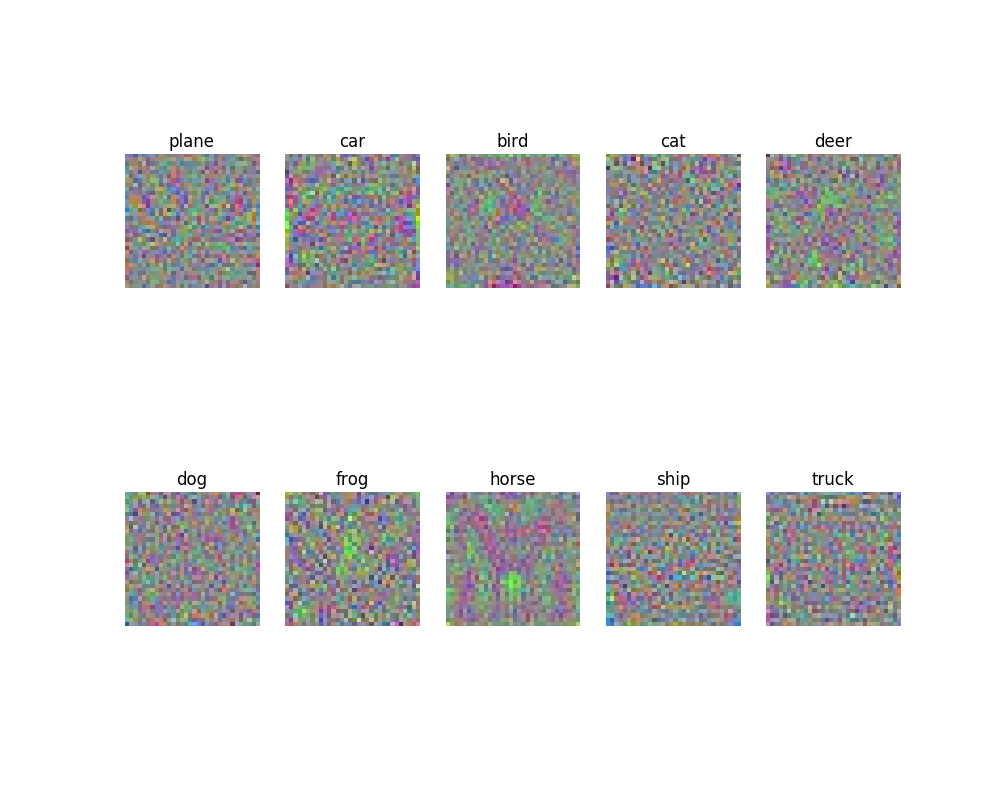
\includegraphics[scale=0.5]{classifer.png}
\end{figure}





\section{Prob 3.2 softmatrix} 
\subsection{loss function}

\begin{lstlisting}  
  gradtemp=np.zeros_like(theta.T)
  k=max(y)
  do=0.0
  for j in range(0,m):
    do=sum(np.exp(X[j].dot(theta)))
    so=np.exp(X[j].dot(theta.T[y[j]]))
    J-= np.log(so/do)
    for i in range(0,k+1):
      so2=np.exp(X[j].dot(theta.T[i]))
      gradtemp[i]-=[-so2/do]*X[j]
      if y[j]==i:
        gradtemp[i]-=[1.0]*X[j]
  J=(J+reg/2*np.sum(np.square(theta)))/m
\end{lstlisting}  

\section{Prob 3.3 softmatrix gradient of loss funciton} 


loss: (should be close to 2.38):  2.35469072576
\subsection{check it with numerical gradients}
here is the result:
\begin{lstlisting} 
numerical: 0.129160 analytic: 0.129160, relative error: 3.928971e-07
numerical: 1.741081 analytic: 1.741081, relative error: 5.696998e-08
numerical: 1.263609 analytic: 1.263608, relative error: 3.495037e-08
numerical: 1.147649 analytic: 1.147649, relative error: 2.377169e-08
numerical: -0.381516 analytic: -0.381516, relative error: 4.228033e-09
numerical: -0.712344 analytic: -0.712344, relative error: 2.496421e-08
numerical: 3.929318 analytic: 3.929318, relative error: 1.349814e-08
numerical: -1.199223 analytic: -1.199223, relative error: 1.557115e-08
numerical: 0.475819 analytic: 0.475818, relative error: 8.416700e-08
numerical: 0.191925 analytic: 0.191925, relative error: 4.228960e-07
naive loss: 2.343315e+00 computed in 18.502869s\end{lstlisting} 


\subsection{prob 3.4 loss function vectorized version}
\begin{lstlisting} 
  num_train = X.shape[0]
  scores = np.dot(X, theta)
  exp_scores = np.exp(scores)
  prob_scores = exp_scores/np.sum(exp_scores, axis=1, keepdims=True)
  correct_log_probs = -np.log(prob_scores[range(num_train), y])
  J = np.sum(correct_log_probs)
  J/= num_train
  J += 0.5 * reg * np.sum(theta**2)/m

  dscores = prob_scores
  dscores[range(num_train), y] -= 1
  grad = np.dot(X.T, dscores)
  grad/= num_train
  grad += reg * theta/m
\end{lstlisting} 
vectorized loss: 2.308316e+00 computed in 0.531210s
Loss difference: 0.000000
\subsection{prob 3.5 loss function vectorized version}
Loss difference: 0.000000
Gradient difference: 0
\subsection{prob 3.6 minibatch}
\begin{lstlisting} 
train:
   index=np.random.choice(range(0,len(y)),size=batch_size)
      X_batch=X[index,:]
      y_batch=y[index]
\end{lstlisting} 
\begin{lstlisting} 
predict:
  y_pred=np.argmax(X.dot(self.theta),1)
\end{lstlisting} 

\subsection{prob 3.7 select lambda and lr}
\begin{lstlisting} 
for lr in learning_rates:
    for rs in regularization_strengths:
        print("calculating: lr=%e,reg=%e"%(lr,rs))
        ns=best_softmax
        ns.train(X_train,y_train,lr,rs,verbose=True,batch_size=400,num_iters=4000)
        ta=np.mean(y_train == ns.predict(X_train))
        va=np.mean(y_val == ns.predict(X_val))
        results[lr,rs]=(ta,va)
        if va>best_val:
            best_val=va
            best_softmax=ns
\end{lstlisting} 
I find the best value:
lr=1.000000e-06 
reg=5.000000e+04
\subsection{prob 3.8 Training with the best value}
\begin{lstlisting} 
Here is the training result:
iteration 0 / 4000: loss 6.090312
iteration 400 / 4000: loss 3.346101
iteration 800 / 4000: loss 2.402607
iteration 1200 / 4000: loss 1.978008
iteration 1600 / 4000: loss 1.842736
iteration 2000 / 4000: loss 1.794119
iteration 2400 / 4000: loss 1.929885
iteration 2800 / 4000: loss 1.751489
iteration 3200 / 4000: loss 1.868067
iteration 3600 / 4000: loss 1.861193
softmax on raw pixels final test set accuracy: 0.403800
[[468  54  59  20  18  19  30  37 221  74]
 [ 59 485  13  30  26  41  50  34 104 158]
 [100  53 234  70 143  75 179  59  62  25]
 [ 43  73  88 236  57 194 139  43  58  69]
 [ 59  39 103  50 326  76 194  84  40  29]
 [ 43  45  90 132  83 336 104  62  76  29]
 [ 16  54  68  83 108  76 508  21  28  38]
 [ 48  50  56  54 115  75  64 392  55  91]
 [144  68   8  15   8  54   9  13 573 108]
 [ 66 171   9  26  19  17  50  43 119 480]]
\end{lstlisting} 

\subsection{visualizing the learned  matrix}
\begin{figure}
  \caption{Visualization of CIFAR-10 $\theta$s}
  \centering
   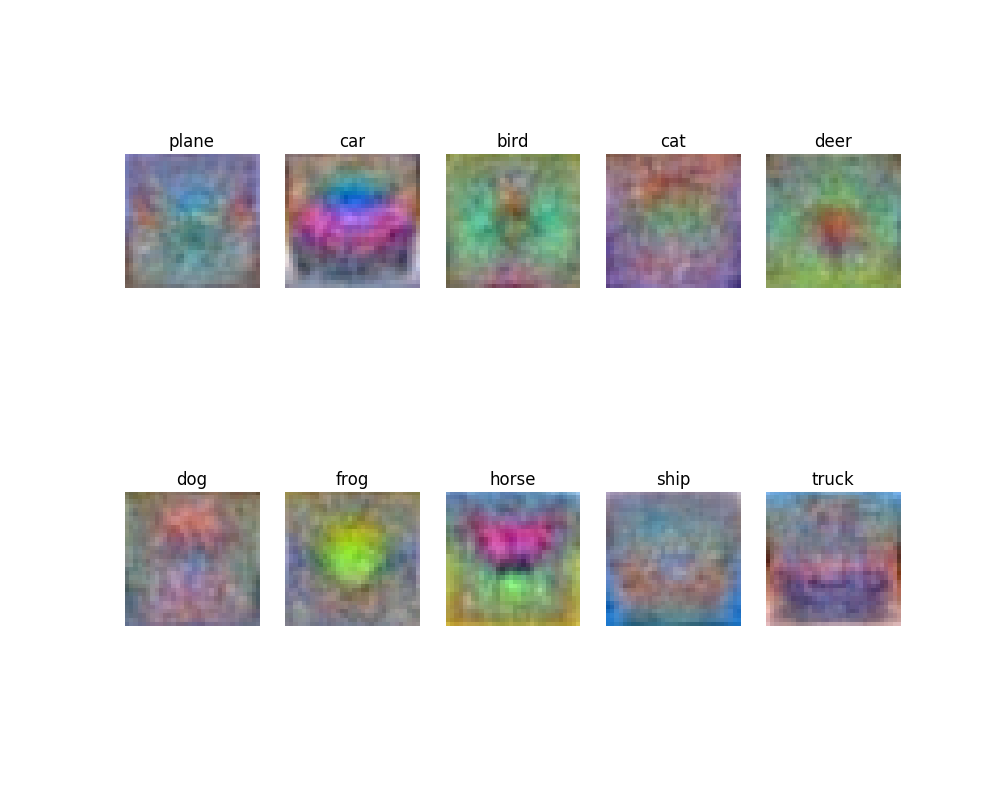
\includegraphics[scale=0.5]{classifernew.png}
\end{figure}
When comparing the confusion matrix
\begin{lstlisting} 
[[468  54  59  20  18  19  30  37 221  74]
 [ 59 485  13  30  26  41  50  34 104 158]
 [100  53 234  70 143  75 179  59  62  25]
 [ 43  73  88 236  57 194 139  43  58  69]
 [ 59  39 103  50 326  76 194  84  40  29]
 [ 43  45  90 132  83 336 104  62  76  29]
 [ 16  54  68  83 108  76 508  21  28  38]
 [ 48  50  56  54 115  75  64 392  55  91]
 [144  68   8  15   8  54   9  13 573 108]
 [ 66 171   9  26  19  17  50  43 119 480]]
\end{lstlisting} 


\begin{lstlisting}    
The old confusion matrix is 
[[460  61  22  27  19  34  26  60 207  84]
 [ 64 459  18  33  26  29  47  53  94 177]
 [122  64 199  77  93  91 145  87  75  47]
 [ 68  85  80 161  49 187 168  48  70  84]
 [ 65  44 100  61 237  81 200 129  34  49]
 [ 51  70  80 130  83 270 112  86  64  54]
 [ 32  53  66  95  89  75 459  54  30  47]
 [ 51  67  51  47  68  85  64 400  51 116]
 [144  82   9  23  10  31  25  19 542 115]
 [ 60 198  11  23  23  28  56  62 113 426]]
\end{lstlisting}    
Most classifiers are better than the old one, except the horse.
Many ships are predicted as deer. As we can see the horse and deer have very similar average picture. They are all tall animals with 4 legs.




\subsection{extra}
code for changing iteration:
\begin{lstlisting}  
lr=1.000000e-06 
reg=5.000000e+04
ns=best_softmax
results = {};
b=400
csize=[400,800,2000,8000]
x=[]
y=[]
z=[]
for c in csize:
    ns.train(X_train,y_train,lr,rs,verbose=True,batch_size=b,num_iters=c)
    y_test_pred = best_softmax.predict(X_test)
    test_accuracy = np.mean(y_test == y_test_pred)
    x.append(c)
    y.append(test_accuracy)
    
plt.plot(x,y,"o")

plt.savefig("classiferitere")
\end{lstlisting}  

code for changing batch size
\begin{lstlisting} 
lr=1.000000e-06 
reg=5.000000e+04
ns=best_softmax
results = {};
bsize=[400,1000,2000]
c=2000
x=[]
y=[]
z=[]
for b in bsize:
    ns.train(X_train,y_train,lr,rs,verbose=True,batch_size=b,num_iters=c)
    y_test_pred = best_softmax.predict(X_test)
    test_accuracy = np.mean(y_test == y_test_pred)
    x.append(b)
    y.append(test_accuracy)
    
plt.plot(x,y,"o")
plt.savefig("classiferbatch")
\end{lstlisting} 

\begin{figure}[H]
  \caption{batch size performance $\theta$s}
  \centering
    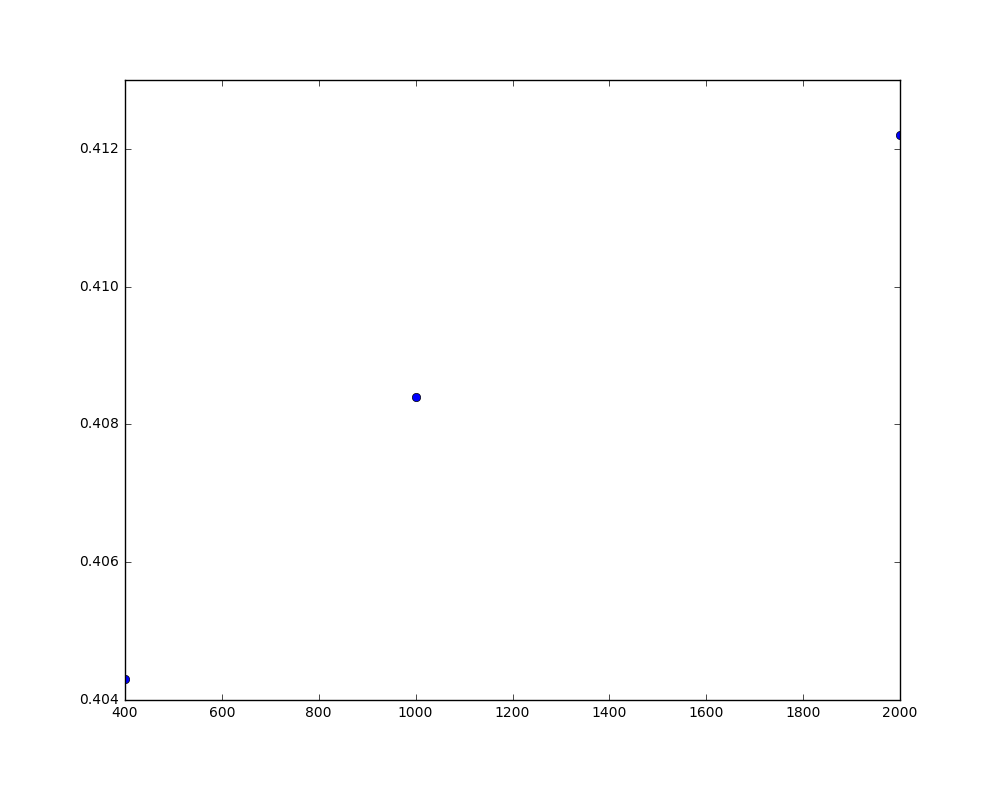
\includegraphics[scale=0.5]{classiferbatch.png}
\end{figure}
\begin{figure}[H]
  \caption{iteration size performance $\theta$s}
  \centering
    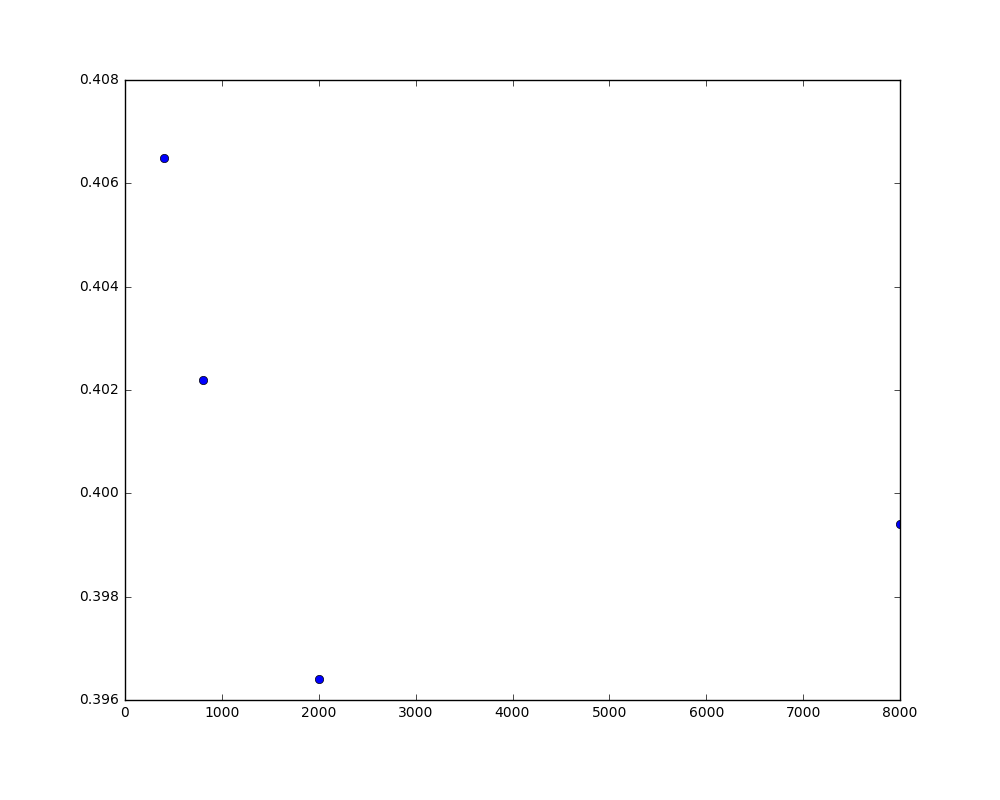
\includegraphics[scale=0.5]{classiferitere.png}
\end{figure}
Based on our runs, increasing the batch size can increase the performance. However increasing the iteration size to much may cause a problem of overfitting. The classifier have a larger possibility to learn the same data again and again, which will make the prediction less accurate. When we increase the iteration size, we need to make sure we increase the regularization parameter as well to avoid the overfitting problem and more heavily penalize larger parameter values. 
In general, high iterations and batch size coupled with low learning rates will yield the best accuracy. The regularization parameter must scale accordingly with the batch size. 


\subsection{prob 3.10 compare ova with softmax}
\begin{lstlisting}   
	soft	ova
plane	468	460
car	485	459
bird	234	199
cat	236	161
deer	326	237
dog	336	270
frog	508	459
horse	392	400
ship	573	542
truck	480	426
\end{lstlisting}   

Usually the softmatrix have better performance. This is because when calculating the relative possibility, the softmatrix makes all the possibilities coupled together so the updating process will change slowly, which gives more stable result.


















\end{document}
